\documentclass[8pt]{extarticle}
\title{}
\author{Avinash Iyer}
\date{}

%font setup
%
%\usepackage[math]{anttor}

%paper setup
\usepackage{geometry}
\geometry{letterpaper, portrait, margin=1in}
\usepackage{fancyhdr}

%symbols
\usepackage{amsmath}
\usepackage{amssymb}
\usepackage{hyperref}
\usepackage{gensymb}

\usepackage[T1]{fontenc}
\usepackage[utf8]{inputenc}

%chemistry stuff
\usepackage[version=4]{mhchem}
\usepackage{chemfig}

%plotting
\usepackage{pgfplots}
\usepackage{tikz}

%\usepackage{natbib}

%graphics stuff
\usepackage{graphicx}
\graphicspath{ {./images/} }

%a useful command
\newcommand{\plain}[1]{\textrm{#1}}

%code stuff
%when using minted, make sure to add the -shell-escape flag
%you can use lstlisting if you don't want to use minted
%\usepackage{minted}
%\usemintedstyle{pastie}
%\newminted[javacode]{java}{frame=lines,framesep=2mm,linenos=true,fontsize=\footnotesize,tabsize=3,autogobble,}
%\newminted[cppcode]{cpp}{frame=lines,framesep=2mm,linenos=true,fontsize=\footnotesize,tabsize=3,autogobble,}

\usepackage{listings}
\usepackage{color}
\definecolor{dkgreen}{rgb}{0,0.6,0}
\definecolor{gray}{rgb}{0.5,0.5,0.5}
\definecolor{mauve}{rgb}{0.58,0,0.82}

\lstset{frame=tb,
	language=Java,
	aboveskip=3mm,
	belowskip=3mm,
	showstringspaces=false,
	columns=flexible,
	basicstyle={\small\ttfamily},
	numbers=none,
	numberstyle=\tiny\color{gray},
	keywordstyle=\color{blue},
	commentstyle=\color{dkgreen},
	stringstyle=\color{mauve},
	breaklines=true,
	breakatwhitespace=true,
	tabsize=3
}
\pagestyle{fancy}
\fancyhf{}
\rhead{Avinash Iyer, Tobias Searcy-Jorgensen}
\lhead{Lab 7: Ballistic Pendulum}
\begin{document}{
\section*{Abstract}
In this lab, we tested two different experiments using a spring cannon to calculate initial speed of a steel ball ejected from the cannon. In the first experiment, we shot the steel ball into a ballistic pendulum's cage, which then pushed an angle marker to the maximum height that the ballistic pendulum reached. We performed this experiment 12 times\textendash 4 times each at each compression mode of short range, medium range, and long range. In the second experiment, we used a photogate timer to measure how much time it took for the steel ball to pass through the photogate after it was shot out of the cannon. We performed this experiment three times for each of the compression modes. In the first experiment, we found that the steel ball exiting the cannon at the short range setting was moving at $2.36\pm 0.02$ m/s, consistent with the calculation in the second experiment of $2.4\pm 0.1$ m/s. For the medium range mode, the steel ball in the first experiment was found to move at $3.71\pm 0.03$ m/s, consistent with the calculation in the second experiment of $3.7\pm 0.1$. For the long range mode, the steel ball was found to move at $5.41\pm 0.05$ m/s in the first experiment, consistent with the calculation in the second experiment of $5.1\pm 0.1$ m/s. After calculating these speeds, the fraction of energy lost due to heat after the collision of the ball with the cage was found to be around $79\%$, which is consistent with the theoretical value of $78.5\%$. Finally, we calculated the spring constant using the values from the second experiment\textendash despite the existence of two outliers, we found a very consistent value of $320$ N/m for the cannon's spring constant.
\section*{Experiment 1}
\subsection*{Part 1}
A spring cannon with three compression modes is set up at the base of a ballistic pendulum with an angle marker on the wall behind the pendulum. The pendulum can lock a $25$mm steel ball inside. The ball and ball + cage are measured with a triple beam balance. When the apparatus is set up with the steel ball in the spring cannon set to the desired compression mode ($x_1$, $x_2$, or $x_3$), the angle marker on the ballistic pendulum is moved towards the $0$ degree line, then the spring cannon is released. The ballistic pendulum moves the angle marker towards the maximum angle it takes. The length of the ballistic pendulum, the angle it takes, and the various masses are included in a formula to find the initial velocity. A visualization is shown below.
\begin{center}
	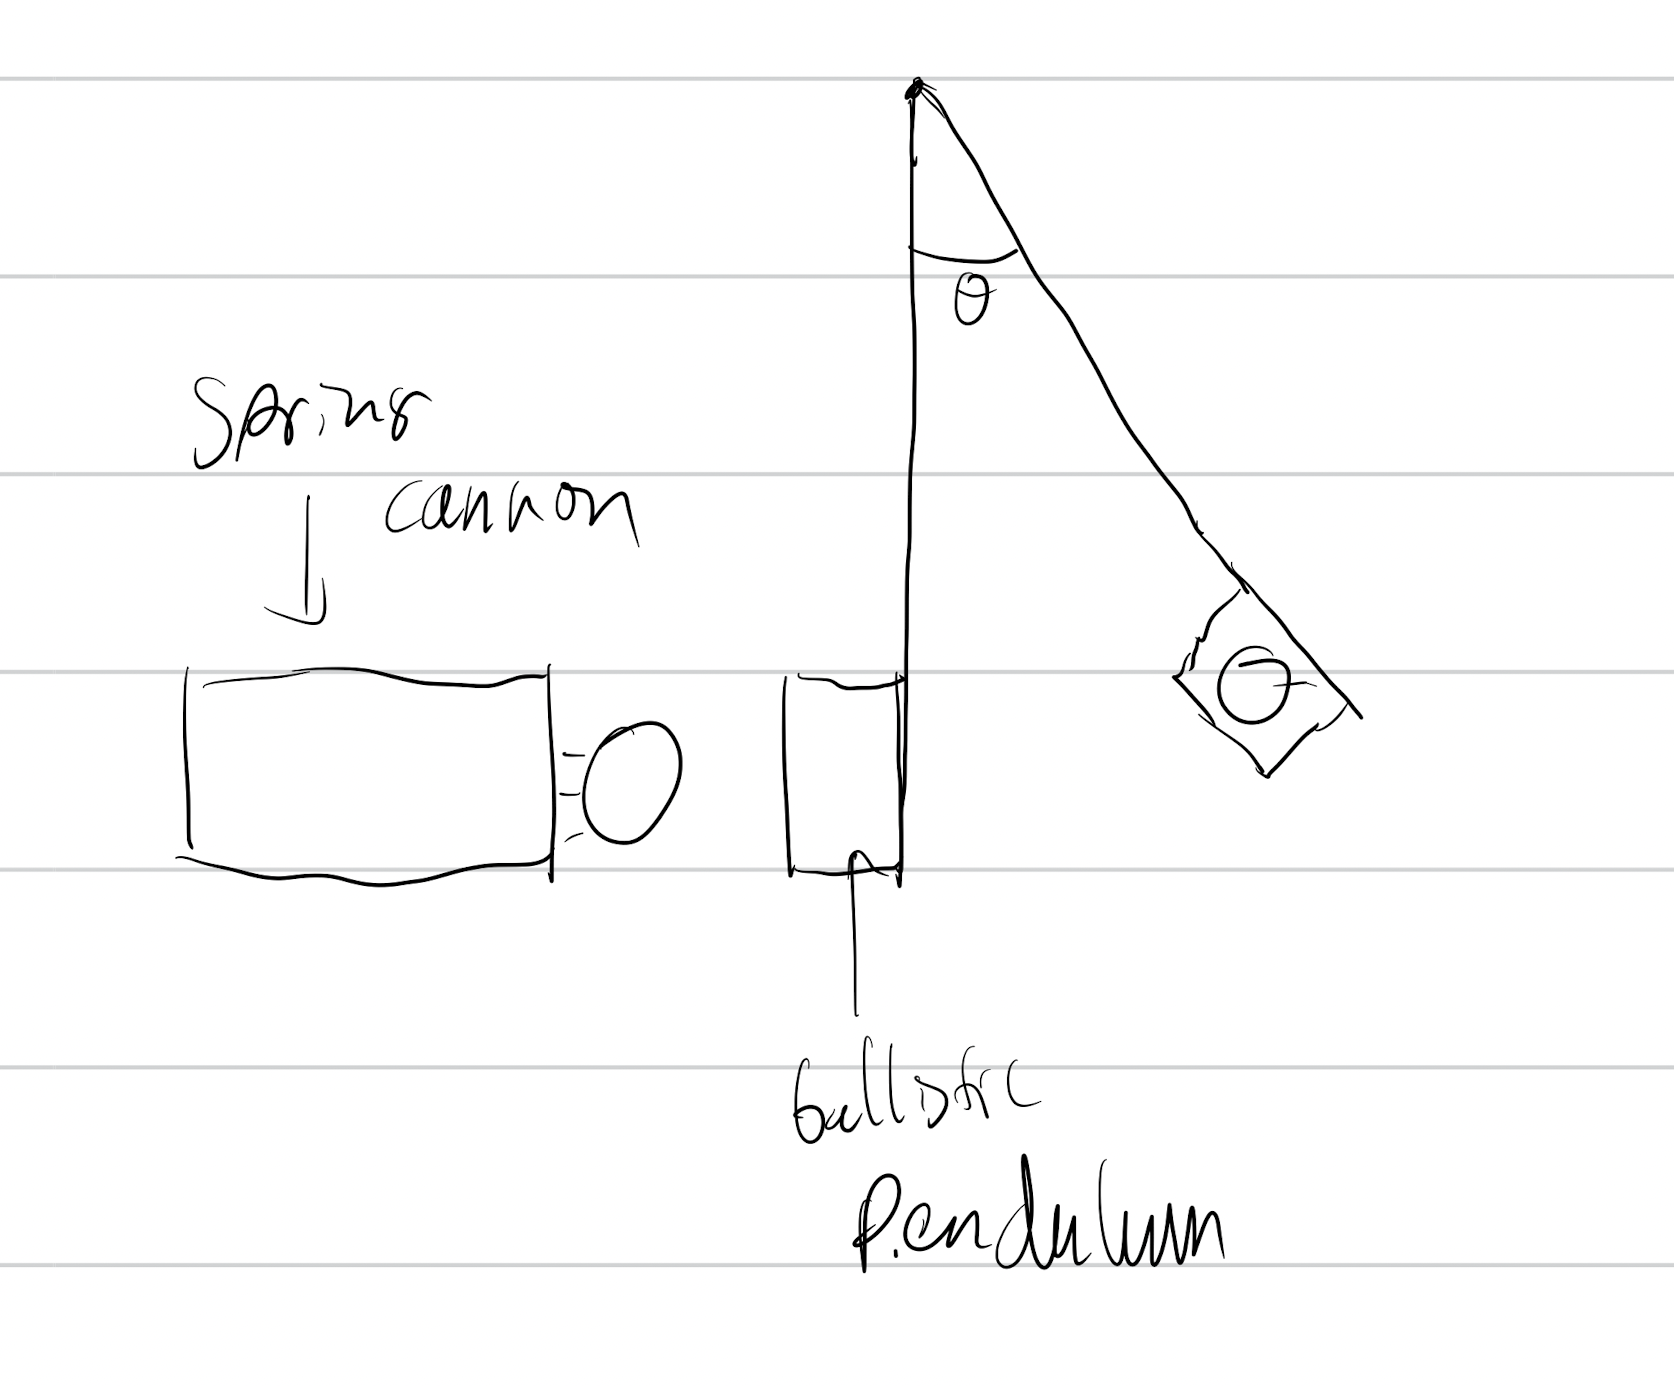
\includegraphics[width=10cm]{Lab7Image1}
\end{center}
\subsection*{Part 2}
Working backwards, we found the height that the ballistic pendulum took from the angle using $h = l(1-\cos\theta)$. Then, the potential energy of the ball + cage combination is equal to $(m+M)gh$, which is equal by conservation of kinetic energy to $(1/2)(m+M)(v_{(m+M)i})^2$. Then, we use conservation of momentum assuming a perfectly inelastic collision to find $v_{(m+M)i} = \frac{m}{m+M}v_{i}$. Combining all these values together, we get that $v_i = \frac{(m+M)\sqrt{2gl(1-\cos\theta}}{m}$.
\subsection*{Part 3}
\begin{itemize}
	\item We are assuming that the ballistic pendulum is a point mass on the end of a string rather than a rigid lever arm. The fact that the ballistic pendulum is a lever arm increases the necessary mechanical energy to reach a given height, meaning our experimental value of $v_i$ is lower than the actual value.
	\item We are assuming that there is no other loss of mechanical energy from sound, heat, etc while the pendulum is moving. Accounting for these would make the experimental value of $v_i$ lower than the actual value.
\end{itemize}
\subsection*{Part 4}
\begin{itemize}
	\item Angle measurements: we are keeping experimental uncertainty on angle measurements low by carrying out multiple trials. Additionally, we start by putting the angle indicator somewhat close to the final value of the ballistic pendulum.
	\item Mass measurements: we are reducing the uncertainty in measuring the masses of the various objects by using a triple beam balance that measures to the nearest $0.1$ grams, as opposed to digital scales that measure to the nearest $1$ gram.
	\item Length measurements: we used a meterstick and ruler to measure to the nearest $0.001$ meters for both the spring's displacement and the length of the pendulum.
\end{itemize}
\subsection*{Part 5}
\begin{center}
	\renewcommand{\arraystretch}{1.5}
	\begin{tabular}{c|c}
		Value & Measurement\\
		\hline
		Ball + Cage & $307.3\pm 0.1$g\\
		Washer & $6.3\pm 0.1$g\\
		Ball + Washer & $72.4\pm 0.1$g\\
		Ball & $66.1\pm 0.1$g\\
		Cage & $241.2\pm 0.1$g\\
		Pendulum Length & $0.280\pm 0.001$m\\
		$x_1$ & $0.034\pm 0.001$m\\
		$x_2$ & $0.054\pm 0.001$m\\
		$x_3$ & $0.075\pm 0.001$m
	\end{tabular} \\
	\begin{tabular}{c|c|c}
		Trial (Displacement Mode) & Angle (degrees) & Initial Velocity (m/s)\\
		\hline
		1 $(x_1)$ & $18.0\pm 0.5$ & $2.41\pm 0.04$ \\
		2 $(x_1)$ & $17.5\pm 0.5$ & $2.34\pm 0.04$ \\
		3 $(x_1)$ & $17.0\pm 0.5$ & $2.27\pm 0.04$ \\
		4 $(x_1)$ & $18.0 \pm 0.5$ & $2.41\pm 0.04$ \\
		\hline
		5 $(x_2)$ & $28.0\pm 0.5$ & $3.73\pm 0.07$\\
		6 $(x_2)$ & $27.5\pm 0.5$ & $3.66\pm 0.07$\\
		7 $(x_2)$ & $28.0\pm 0.5$ & $3.73\pm 0.07$\\
		8 $(x_2)$ & $28.0\pm 0.5$ & $3.73\pm 0.07$\\
		\hline
		9 $(x_3)$ & $39.0\pm 0.5$ & $5.14\pm 0.1$\\
		10 $(x_3)$ & $39.0\pm 0.5$ & $5.14\pm 0.1$\\
		11 $(x_3)$ & $39.0\pm 0.5$ & $5.14\pm 0.1$\\
		12 $(x_3)$ & $39.0\pm 0.5$ & $5.14\pm 0.1$\\
	\end{tabular}
\end{center}
\subsection*{Part 6}
\subsubsection*{Subpart A}
To calculate the initial speed, we used the formula found in Part 2, with $v_{i} = \frac{(m+M)\sqrt{2gl(1-\cos\theta)}}{m}$. In the case of $x_1$, the first spring compression mode, we found a velocity of $2.41\pm 0.04$ in the first trial where $\theta = 18.0\pm 0.5^\circ$.
\subsubsection*{Subpart B}
The error propagation in the case of the first measurement and first set of compression modes is shown below. The results are rounded here, but were not rounded until the final results in the Excel sheet.
\begin{align*}
	\theta &= 18.0\\
	\delta\theta &= 0.5 \\
	\cos\theta &= 0.951\\
	\delta(\cos\theta) &= \left|\frac{\cos(\theta+\delta\theta) - \cos(\theta-\delta\theta)}{2}\right| \\
	&= 0.003\\
	l &= 0.28\\
	\delta l &= 0.01\\
	h &= l(1-\cos\theta) \\
	&= 0.0137\\
	\delta h &= h\sqrt{\left(\frac{\delta l}{l}\right)^2 + \left(\frac{\delta(\cos\theta)}{\cos\theta}\right)^2}\\
	&=0.004\\
	\sqrt{2gh} &= 0.518 \\
	\delta\sqrt{2gh} &= \frac{\left(\delta h\right)\left(\sqrt{2g}\right)}{2 \sqrt{h}} \\
	&= 0.009\\
	(m+M)\sqrt{2gh} &= 159\\
	\delta \left((m+M)\sqrt{2gh}\right) &= (m+M)\sqrt{2gh}\sqrt{\left(\frac{\delta(m+M)}{m+M}\right)^2 + \left(\frac{\delta \sqrt{2gh}}{\sqrt{2gh}} \right)^2} \\
	&= 3\\
	v_{i_1} &= \frac{(m+M)\sqrt{2gh}}{m} \\
	 &= 2.41\\
	\delta \left(\frac{(m+M)\sqrt{2gh}}{m}\right) &= \frac{(m+M)\sqrt{2gh}}{m}\sqrt{\left(\frac{\delta \left((m+M)\sqrt{2gh}\right)}{(m+M)\sqrt{2gh}}\right)^2 + \left(\frac{\delta m}{m}\right)^2} \\
	&= 0.04\\
	v_{1} &= \frac{v_{i_1} + v_{i_2} + v_{i_3} + v_{i_4}}{4}\\
	&= 2.36 \\
	\delta v_{1} &= \frac{\sqrt{\sum\limits_{k=1}^{4} \delta v_{i_{k}}^2}}{4} \\
	&= 0.02 \\
	v_{1} &= 2.36\pm 0.02~\plain{m/s}
\end{align*}
\subsubsection*{Subpart C}
\begin{center}
	\renewcommand{\arraystretch}{1.5}
	\begin{tabular}{c|c}
		Compression Mode & Velocity (m/s) \\
		\hline
		$x_1$ & $2.36\pm 0.02$ \\
		$x_2$ & $3.71\pm 0.03$ \\
		$x_3$ & $5.14 \pm 0.05$
	\end{tabular}
\end{center}
\section*{Experiment 2}
\subsection*{Part 1}
A photogate was set up about 5 centimeters from the edge of the spring cannon, with a box on one end to catch the steel ball as it left the chamber of the spring cannon. The steel ball has a known diameter of $25$ centimeters. When the steel ball is launched from the spring cannon, the photogate measures the time that the ball spends blocking the photogate's laser sensor, yielding a certain time $t$. Trials are repeated three times at each compression mode for the sake of accuracy. A visualization is shown below.
\begin{center}
	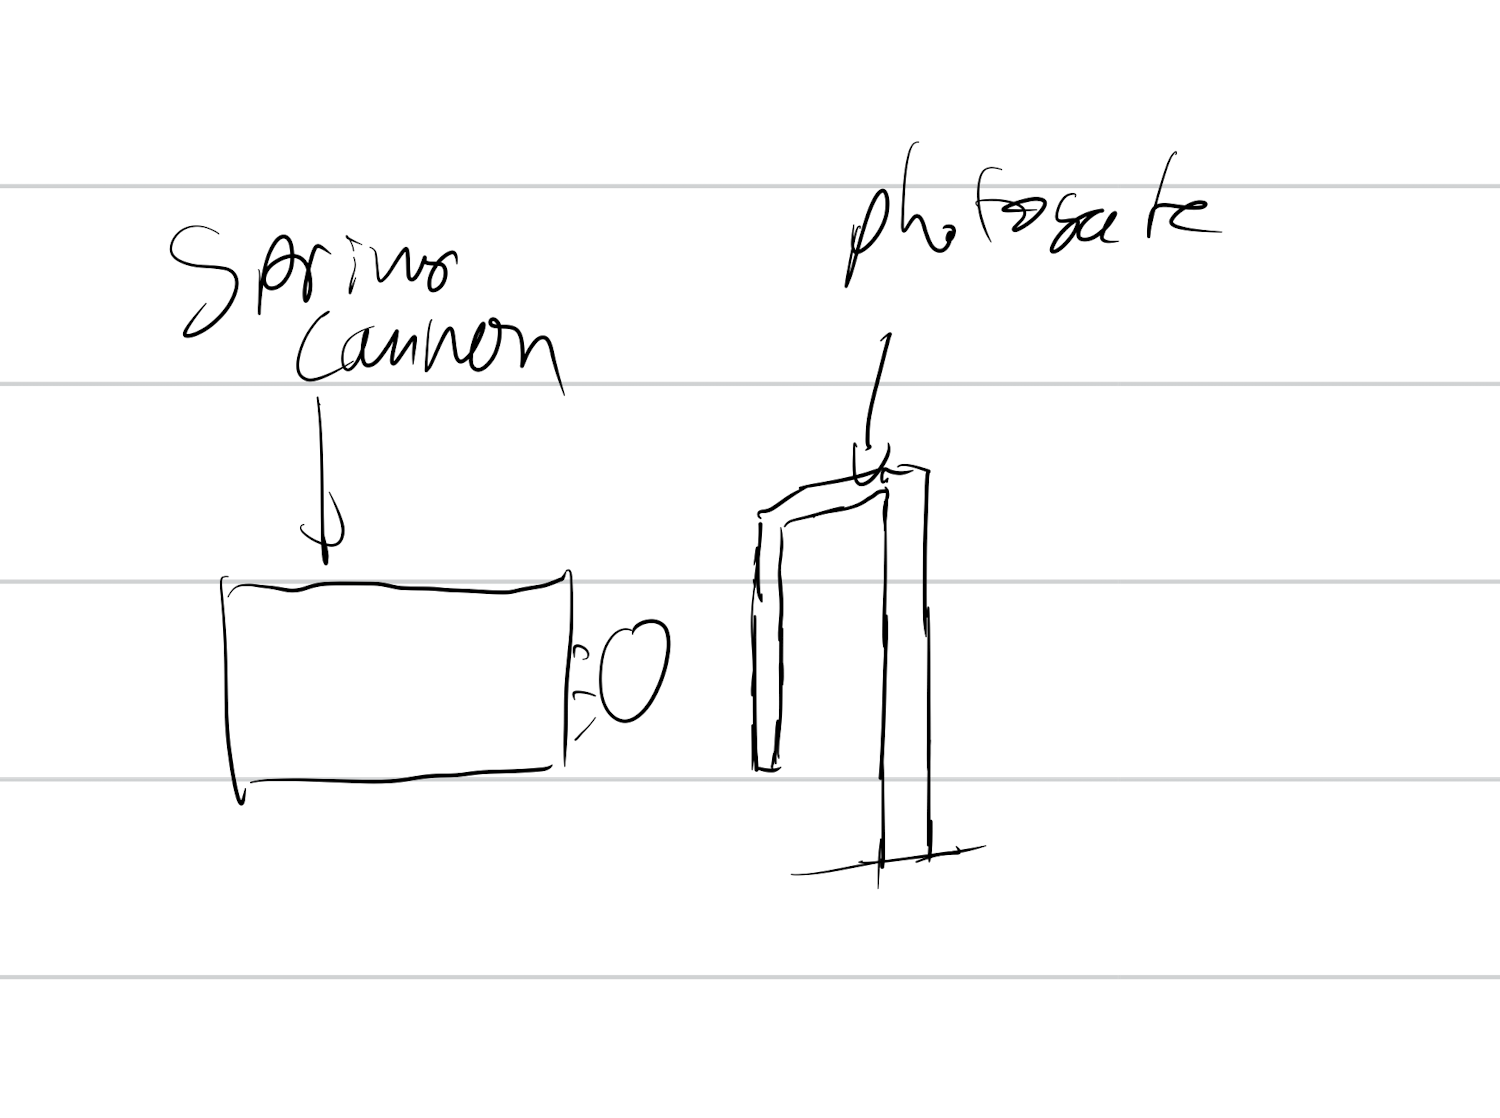
\includegraphics[width=10cm]{Lab7Image2}
\end{center}
\subsection*{Part 2}
We divided the known width of the ball ($25$ cm) by the time measured on the photogate to find the speed of the ball.
\subsection*{Part 3}
We are assuming no air resistance or friction from the ball exiting the spring cannon, as well as the ball being at maximum width when it moves through the photogate.
\subsection*{Part 4}
\begin{itemize}
	\item Ball not at maximum width: we carefully positioned the photogate to be such that the laser of the photogate crosses the spring cannon at maximum width.
	\item Instrumental uncertainty: we are using an instrumental uncertainty of $0.1$ milliseconds with the photogate (albeit, for the first experiment, we had an instrumental uncertainty of $1$ millisecond.
	\item Measurement of the ball: we are assuming the ball is $25$ millimeters with $1$mm uncertainty.
\end{itemize}
\subsection*{Part 5}
The values of $x_1,x_2,x_3$ were found in Experiment 1.
\begin{center}
	\renewcommand{\arraystretch}{1.5}
	\begin{tabular}{c|c|c}
		Trial (Compression Mode) & Photogate Measurement (s) & Velocity (m/s)\\
		\hline
		1 ($x_1$) & $0.010\pm 0.001$ & $2.5$\\
		2 ($x_1$) & $0.010\pm 0.001$ & $2.5$\\
		3 ($x_1$) & $0.011\pm 0.001$ & $2.5$\\
		4 ($x_2$) & $0.0067\pm 0.0001$ & $3.7$\\
		5 ($x_2$) & $0.0067\pm 0.0001$ & $3.7$\\
		6 ($x_2$) & $0.0067\pm 0.0001$ & $3.7$\\
		7 ($x_3$) & $0.0049\pm 0.0001$ & $5.1$\\
		8 ($x_3$) & $0.0048\pm 0.0001$ & $5.2$\\
		9 ($x_3$) & $0.0049\pm 0.0001$ & $5.1$
	\end{tabular}
\end{center}
\subsection*{Part 6}
\subsubsection*{Subpart A}
Calculation shown for the first trial below:
\begin{align*}
	v_{1} &= \frac{0.025}{0.010}\\
	&= 2.5~\plain{m/s} 
\end{align*}
\subsubsection*{Subpart B}
\begin{align*}
	w &= 0.025\\
	\delta w &= 0.001\\
	t &= 0.010 \\
	\delta t &= 0.001 \\
	v &= \frac{w}{t}\\
	v &= 2.5 \\
	\delta v &= v\sqrt{\left(\frac{\delta w}{2}\right)^2 + \left(\frac{\delta t}{t}\right)^2} \\
	&= 0.3\\
	v_{1} &= \frac{v_{i_1} + v_{i_2} + v_{i_3}}{3}\\
	&= 2.4\\
	\delta v_1 &= \frac{\sqrt{\left(\frac{\delta v_{i_1}}{v_{i_1}}\right)^2 + \left(\frac{\delta v_{i_2}}{v_{i_2}}\right)^2 + \left(\frac{\delta v_{i_3}}{v_{i_3}}\right)^2}}{3} \\
	&= 0.1 
\end{align*}
\subsubsection*{Subpart C}
\begin{center}
	\renewcommand{\arraystretch}{1.5}
	\begin{tabular}{c|c}
		Compression Mode & Average Velocity (m/s) \\
		\hline
		$x_1$ & $2.4\pm 0.1$ \\
		$x_2$ & $3.7\pm 0.1$\\
		$x_3$ & $5.1\pm 0.1$
	\end{tabular}
\end{center}
\section*{Analysis of the Results}
\subsection*{Part 1}
The results are consistent with each other.
\subsection*{Part 2}
\subsubsection*{Subpart A}
Averaging over all trials at each of the compression modes, we get the following results for $E_f$ and $E_i$, where $E_{f}$ is calculated from the final height of the ball and cage combination in Experiment 1 and $E_i$ is calculated from the initial speed in Experiment 2:
\begin{center}
	\begin{tabular}{c|c|c|c}
		Compression Mode & $E_{i}$ & $E_{f}$ & $\frac{E_{i}-E_{f}}{E_{i}}$ \\
		\hline
		$x_1$ & $0.19$ & $0.040$ & $80.\%$\\
		$x_2$ & $0.46$ & $0.098$ & $79\%$ \\
		$x_3$ & $0.87$ & $0.19$ & $78\%$
	\end{tabular}
\end{center}
\subsubsection*{Subpart B}
\begin{align*}
	\frac{\Delta E}{E_{i}} &= 1 - \frac{m}{m+M} \\
	&= 1 - \frac{66.1}{307.3} \\
	&= 78.5\%
\end{align*}
\subsection*{Subpart C}
These values are consistent, meaning that most of our energy loss was due to heat, there was less energy loss due to sound or other extraneous internal energy.
\subsection*{Part 3}
\subsubsection*{Subpart A}
Yes, we do assume that all the potential energy of the spring is converted into kinetic energy of the steel ball.
\subsubsection*{Subpart B}
\begin{center}
	\renewcommand{\arraystretch}{1.5}
	\begin{tabular}{c|c}
		Trial (Compression Mode) & Spring Constant (N/m) \\
		\hline
		1 ($x_1$) & $360$ \\
		2 ($x_1$) & $360$ \\
		3 ($x_1$) & $300$ \\
		4 ($x_2$) & $320$ \\
		5 ($x_2$) & $320$ \\
		6 ($x_2$) & $320$ \\
		7 ($x_3$) & $310$ \\
		8 ($x_3$) & $320$ \\
		9 ($x_3$) & $310$ 
	\end{tabular}
\end{center}
We have two outliers ($>2$ standard deviations) within the first two trials, which is primarily due to having used the photogate uncertainty to the nearest millisecond instead of the nearest 0.1 milliseconds. However, the rest of the spring constant results were consistent within one standard deviation of the mean of $320$ N/m.
}\end{document}